\chapter{Tuning FLEXWIN for your seismograms\label{sec:tuning}}

FLEXWIN is adapted to your specific problem by modifying the values of the parameters in Table~\ref{tb:params}, and the functional form of those parameters that are time-dependent. We consider the algorithm to be correctly adapted when false positives (windows around undesirable features of the seismogram) are minimized, and true positives (window around desirable features) are maximized. The choice of what makes an adequate set of windows remains subjective, as it depends strongly on the quality of the input model, the quality of the data, and the region of the Earth that the tomographic inversion aims to constrain.  

The base values of the various parameters are set in the {\tt PAR\_FILE}, which is read at run time.  Examples of base parameter values for the three tomographic scenarios discussed by \cite{MaggiEtal2009} can be found in Table~\ref{tb:example_params}.  The functional forms of the time dependent parameters may be adjusted by modifying {\tt user\_parameters.f90} (see next section), and re-compiling the code.

\begin{table}[h]
\begin{tabular}{lp{0.8\linewidth}}
\hline
\multicolumn{2}{l}{Standard tuning parameters:} \\[5pt]
$T_{0,1}$     & bandpass filter corner periods \\
$r_{P,A}$     & signal to noise ratios for whole waveform \\
$r_0(t)$      & signal to noise ratios single windows \\
$w_E(t)$      & water level on short-term:long-term ratio \\
$\mathrm{CC}_0(t)$          & acceptance level for normalized cross-correlation\\
$\Delta\tau_0(t)$  & acceptance level for time lag \\
$\Delta\ln{A}_0(t)$   & acceptance level for amplitude ratio \\ 
$\Delta\tau_{\rm ref}$ & reference time lag \\
$\Delta\ln{A}_{\rm ref}$ & reference amplitude ratio \\
\hline
\multicolumn{2}{l}{Fine tuning parameters:} \\ [5pt]
$c_0$ & for rejection of internal minima \\
$c_1$ & for rejection of short windows \\
$c_2$ & for rejection of un-prominent windows \\
$c_{3a,b}$  & for rejection of multiple distinct arrivals \\
$c_{4a,b}$  & for curtailing of windows with emergent starts and/or codas \\
$w_{\mathrm{CC}}\quad w_{\rm len}\quad w_{\rm nwin}$ & for selection of best non-overlapping window combination \\
\hline
\end{tabular}
\caption{\label{tb:params}
Overview of standard tuning parameters, and of fine
tuning parameters.  Values are defined in a parameter file, and the
time dependence of those that depend on time is described by user-defined functions.
} 
\end{table}

\pagebreak
\section{User parameters}
The main user parameters in the {\tt PAR\_FILE} are:
\begin{description}
\item[{\tt WIN\_MIN\_PERIOD}]Corresponds to $T_0$ in Table~\ref{tb:params}, and is the short wavelength cut-off for the band-pass filter applied to the raw synthetic and observed seismograms.
\item[{\tt WIN\_MAX\_PERIOD}]Corresponds to $T_1$ in Table~\ref{tb:params}, and is the long wavelength cut-off for the band-pass filter applied to the raw synthetic and observed seismograms.
\item[{\tt SNR\_INTEGRATE\_BASE}]Corresponds to $r_P$ in Table~\ref{tb:params}, and is the minimum signal to noise ratio on the power of the observed seismogram for windowing to continue.
\item[{\tt SNR\_MAX\_BASE}]Corresponds to $r_A$ in Table~\ref{tb:params}, and is the minimum signal to noise ratio on the modulus of the observed seismogram for windowing to continue.
\item[{\tt WINDOW\_S2N\_BASE}]Corresponds to $r_0$ in Table~\ref{tb:params}, and is the minimum signal to noise ratio for a window on the observed seismogram to be acceptable.
\item[{\tt STALTA\_BASE}]Corresponds to $w_E$ in Table~\ref{tb:params}, and is the water level to be applied to the synthetic short-term/long-term average waveform in order to generate candidate time windows.  See Figure~\ref{fg:win_composite}a.
\item[{\tt CC\_BASE}]Corresponds to $CC_0$ in Table~\ref{tb:params}, and is the minimum normalized cross-correlation value between synthetic and observed seismogram for a window to be acceptable.
\item[{\tt TSHIFT\_BASE}]Corresponds to $\Delta\tau_0$ in Table~\ref{tb:params}, and is the maximum cross-correlation lag (in seconds) between synthetic and observed seismogram for a window to be acceptable.
\item[{\tt DLNA\_BASE}]Corresponds to $\Delta\ln{A}_0$ in Table~\ref{tb:params}, and is the maximum amplitude ratio ($\Delta\ln{A}$ or $\Delta A/A$) between synthetic and observed seismogram for a window to be acceptable.
\item[{\tt TSHIFT\_REFERENCE}]Corresponds to $\Delta\tau_{\rm ref}$ in Table~\ref{tb:params}, and allows for a systematic traveltime bias in the synthetics.
\item[{\tt DLNA\_REFERENCE}]Corresponds to $\Delta\ln{A}_{\rm ref}$ in Table~\ref{tb:params}, and allows for a systematic amplitude bias in the synthetics.
\item[{\tt C\_0}]Corresponds to $C_0$ in Table~\ref{tb:params}, and is expressed as a multiple of $w_E$.  No window may contain a local minimum in its STA:LTA waveform that falls below the local value of $C_0 w_E$.  See Figure~\ref{fg:win_composite}b.
\item[{\tt C\_1}]Corresponds to $C_1$ in Table~\ref{tb:params}, and is expressed as a multiple of $T_0$.  No window may be shorter than $C_1 T_0$.
\item[{\tt C\_2}]Corresponds to $C_2$ in Table~\ref{tb:params}, and is expressed as a multiple of $w_E$.  A window whose seed maximum on the STA:LTA waveform rises less than $C_2 w_E$ above either of its adjacent minima is rejected.  See Figure~\ref{fg:win_composite}c.
\item[{\tt C\_{3a}}]Corresponds to $C_{3a}$ in Table~\ref{tb:params}, and is expressed as a fraction.  It regulates the acceptable height ratio between local maxima in a given window on the STA:LTA waveform.  See Figure~\ref{fg:separation}.
\item[{\tt C\_{3b}}]Corresponds to $C_{3b}$ in Table~\ref{tb:params}, and is expressed as a multiple of $T_0$.  It regulates the acceptable time separation between local maxima in a given window on the STA:LTA waveform.  See Figure~\ref{fg:separation}.
\item[{\tt C\_{4a}}]Corresponds to $C_{4a}$ in Table~\ref{tb:params}, and is expressed as a multiple of $T_0$.  It limits the length of a window before its first local maximum in STA:LTA. 
\item[{\tt C\_{4b}}]Corresponds to $C_{4b}$ in Table~\ref{tb:params}, and is expressed as a multiple of $T_0$.  It limits the length of a window beyond its last local maximum in STA:LTA.  See Figure~\ref{fg:win_composite}d.
\item[{\tt WEIGHT\_AVERAGE\_CC}]Corresponds to $w_{CC}$ in Table~\ref{tb:params}, and is the weight given to the average cross-correlation value in the process of resolving window overlaps. See Figure~\ref{fg:phaseD}.
\item[{\tt WEIGHT\_SPACE\_COVERAGE}]Corresponds to $w_{\rm len}$ in Table~\ref{tb:params}, and is the weight given to the time span covered by windows in the process of resolving window overlaps. 
\item[{\tt WEIGHT\_N\_WINDOWS}]Corresponds to $w_{\rm nwin}$ in Table~\ref{tb:params}, and is the weight given to the total number of windows in the process of resolving window overlaps. 
\end{description}

\begin{table}
\begin{center}
\begin{tabular}{lcccccc}
\hline
			& Global	& \multicolumn{2}{c}{Japan}	& \multicolumn{3}{c}{S. California} \\
\hline
$T_{0,1}$		& 50, 150	& 24, 120 	& 6, 30		& 6, 30		& 3, 30		& 2, 30		\\
$r_{P,A}$		& 3.5, 3.0	& 3.5, 3.0	& 3.5, 3.0	& 3.0, 2.5	& 2.5, 3.5	& 2.5, 3.5	\\
$r_0$			& 2.5		& 1.5		& 3.0		& 3.0		& 4.0		& 4.0		\\
$w_E$			& 0.08		& 0.11		& 0.12		& 0.18		& 0.11		& 0.07		\\
$\mathrm{CC}_0$		& 0.85		& 0.70		& 0.73		& 0.71		& 0.80		& 0.85		\\
$\Delta\tau_0$		& 15		& 12.0		& 3.0		& 8.0		& 4.0		& 3.0		\\
$\Delta\ln{A}_0$	& 1.0 		& 1.0		& 1.5		& 1.5		& 1.0		& 1.0		\\ 
$\Delta\tau_{\rm ref}$	& 0.0		& 0.0		& 0.0		& 4.0		& 2.0 		& 1.0		\\
$\Delta\ln{A}_{\rm ref}$& 0.0		& 0.0		& 0.0		& 0.0		& 0.0		& 0.0		\\
\hline
$c_0$			& 0.7		& 0.7		& 0.7		& 0.7		& 1.3		& 1.0		\\
$c_1$			& 4.0		& 3.0		& 3.0		& 2.0		& 4.0		& 5.0		\\
$c_2$			& 0.3		& 0.0		& 0.6		& 0.0		& 0.0		& 0.0		\\
$c_{3a,b}$		& 1.0, 2.0	& 1.0, 2.0	& 1.0, 2.0	& 3.0, 2.0	& 4.0, 2.5	& 4.0, 2.5	\\
$c_{4a,b}$		& 3.0, 10.0	& 3.0, 25.0	& 3.0, 12.0	& 2.5, 12.0	& 2.0, 6.0	& 2.0, 6.0	\\
$w_{\mathrm{CC}}, w_{\rm len}, w_{\rm nwin}$
			& 1, 1, 1 	& 1, 1, 1	& 1, 1, 1	& 0.5,1.0,0.7	& 0.70,0.25,0.05 & 1,1,1	\\
\hline
\end{tabular}
\caption{\label{tb:example_params}
Values of standard and fine-tuning parameters for the three seismological
scenarios discussed \cite{MaggiEtal2009}.  This table is identical to Table~3 of that study.
} 
\end{center}
\end{table}

\begin{figure}
\center 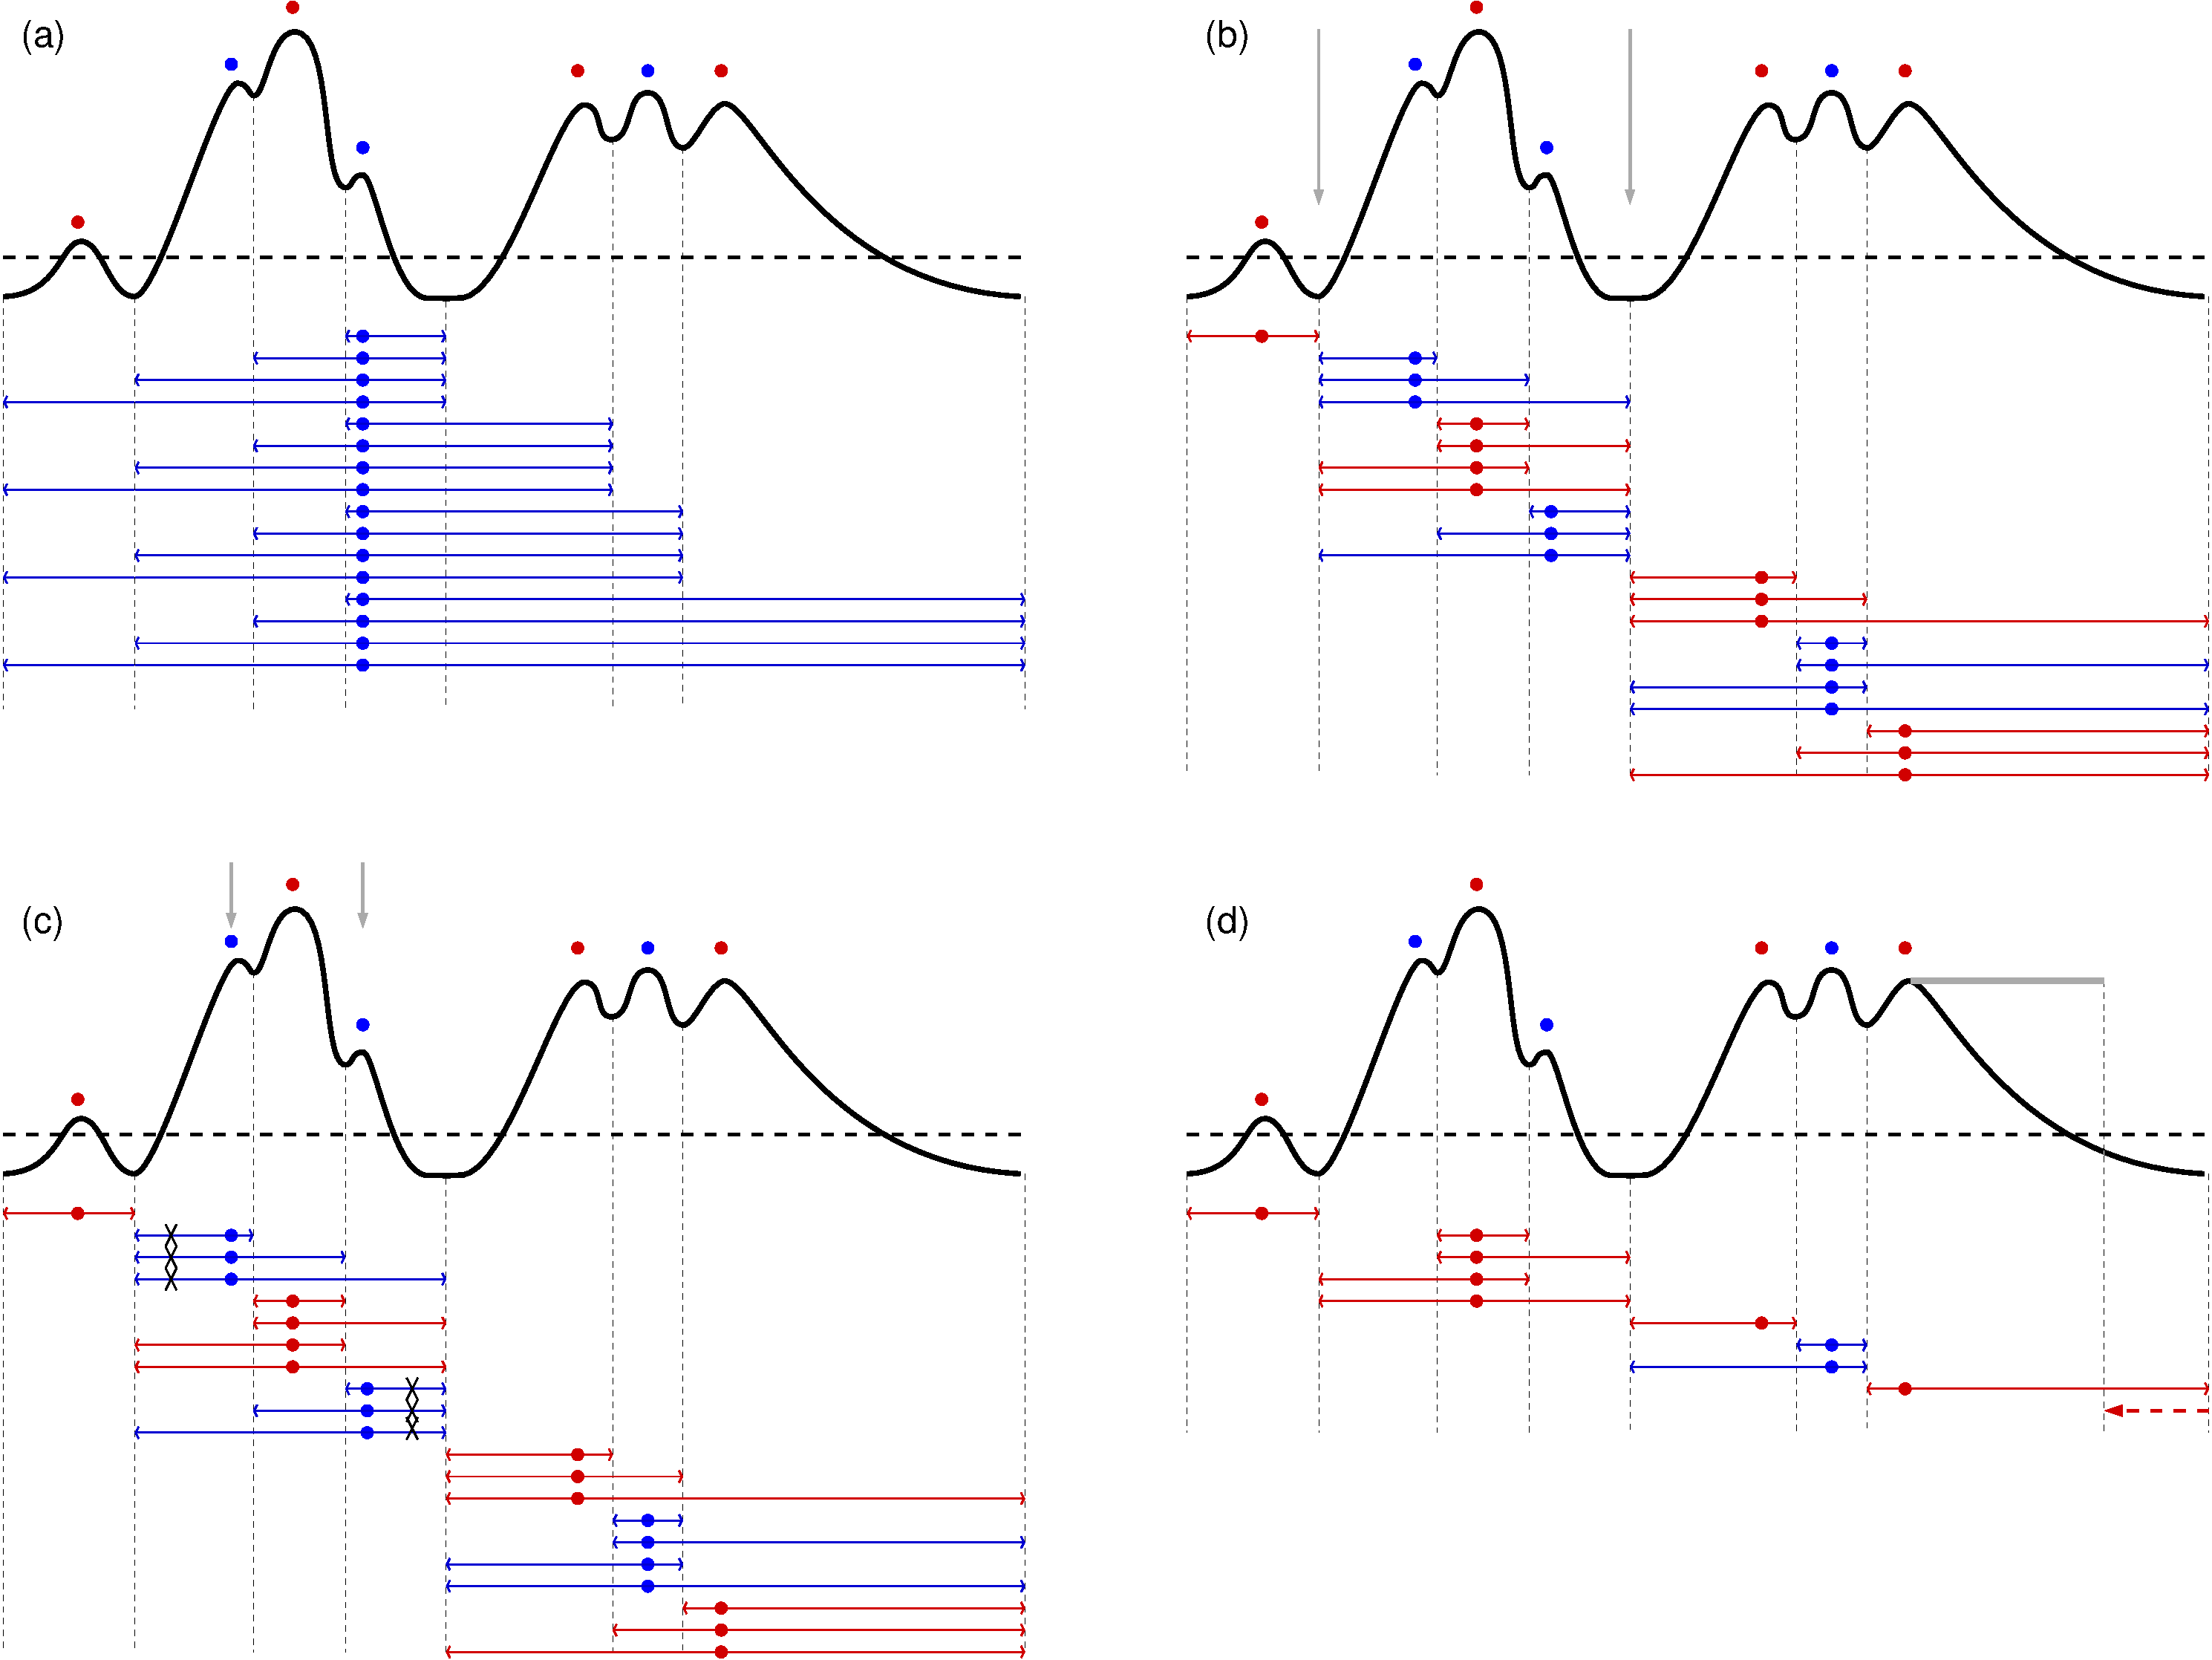
\includegraphics[width=6in]{window_composite.pdf}
\caption{\label{fg:win_composite}
(a)~Window creation process.  The thick black line represents the STA:LTA
waveform $E(t)$, and the thick horizontal dashed line its water level $w_E(t)$.
Local maxima are indicated by alternating red and blue dots, windows are
indicated by two-headed horizontal arrows.  The time of the local maximum used
as the window seed $t_M$ is denoted by the position of the dot. Only windows for the fourth local maximum are shown.  (b)~Rejection of candidate windows based on the amplitude of the local minima.  The two deep
local minima indicated by the grey arrows form virtual barriers. All candidate
windows that cross these barriers are rejected.
(c)~Rejection of candidate
windows based on the prominence of the seed maximum.  The local maxima
indicated by the grey arrows are too low compared to the local minima
adjacent to them.  All windows that have these local maxima as their seed are
rejected (black crosses over the window segments below the time series).
(d)~Shortening of long coda windows.  The grey bar indicates the maximum coda
duration $c_{4b} T_0$.  Note that after the rejection based on prominence represented in (c) and before shortening of long coda windows represented in (d), the algorithm rejects candidate windows based on the separation of distinct phases, a process that is illustrated in Figure~\ref{fg:separation}.
}
\end{figure}

\begin{figure}
\center 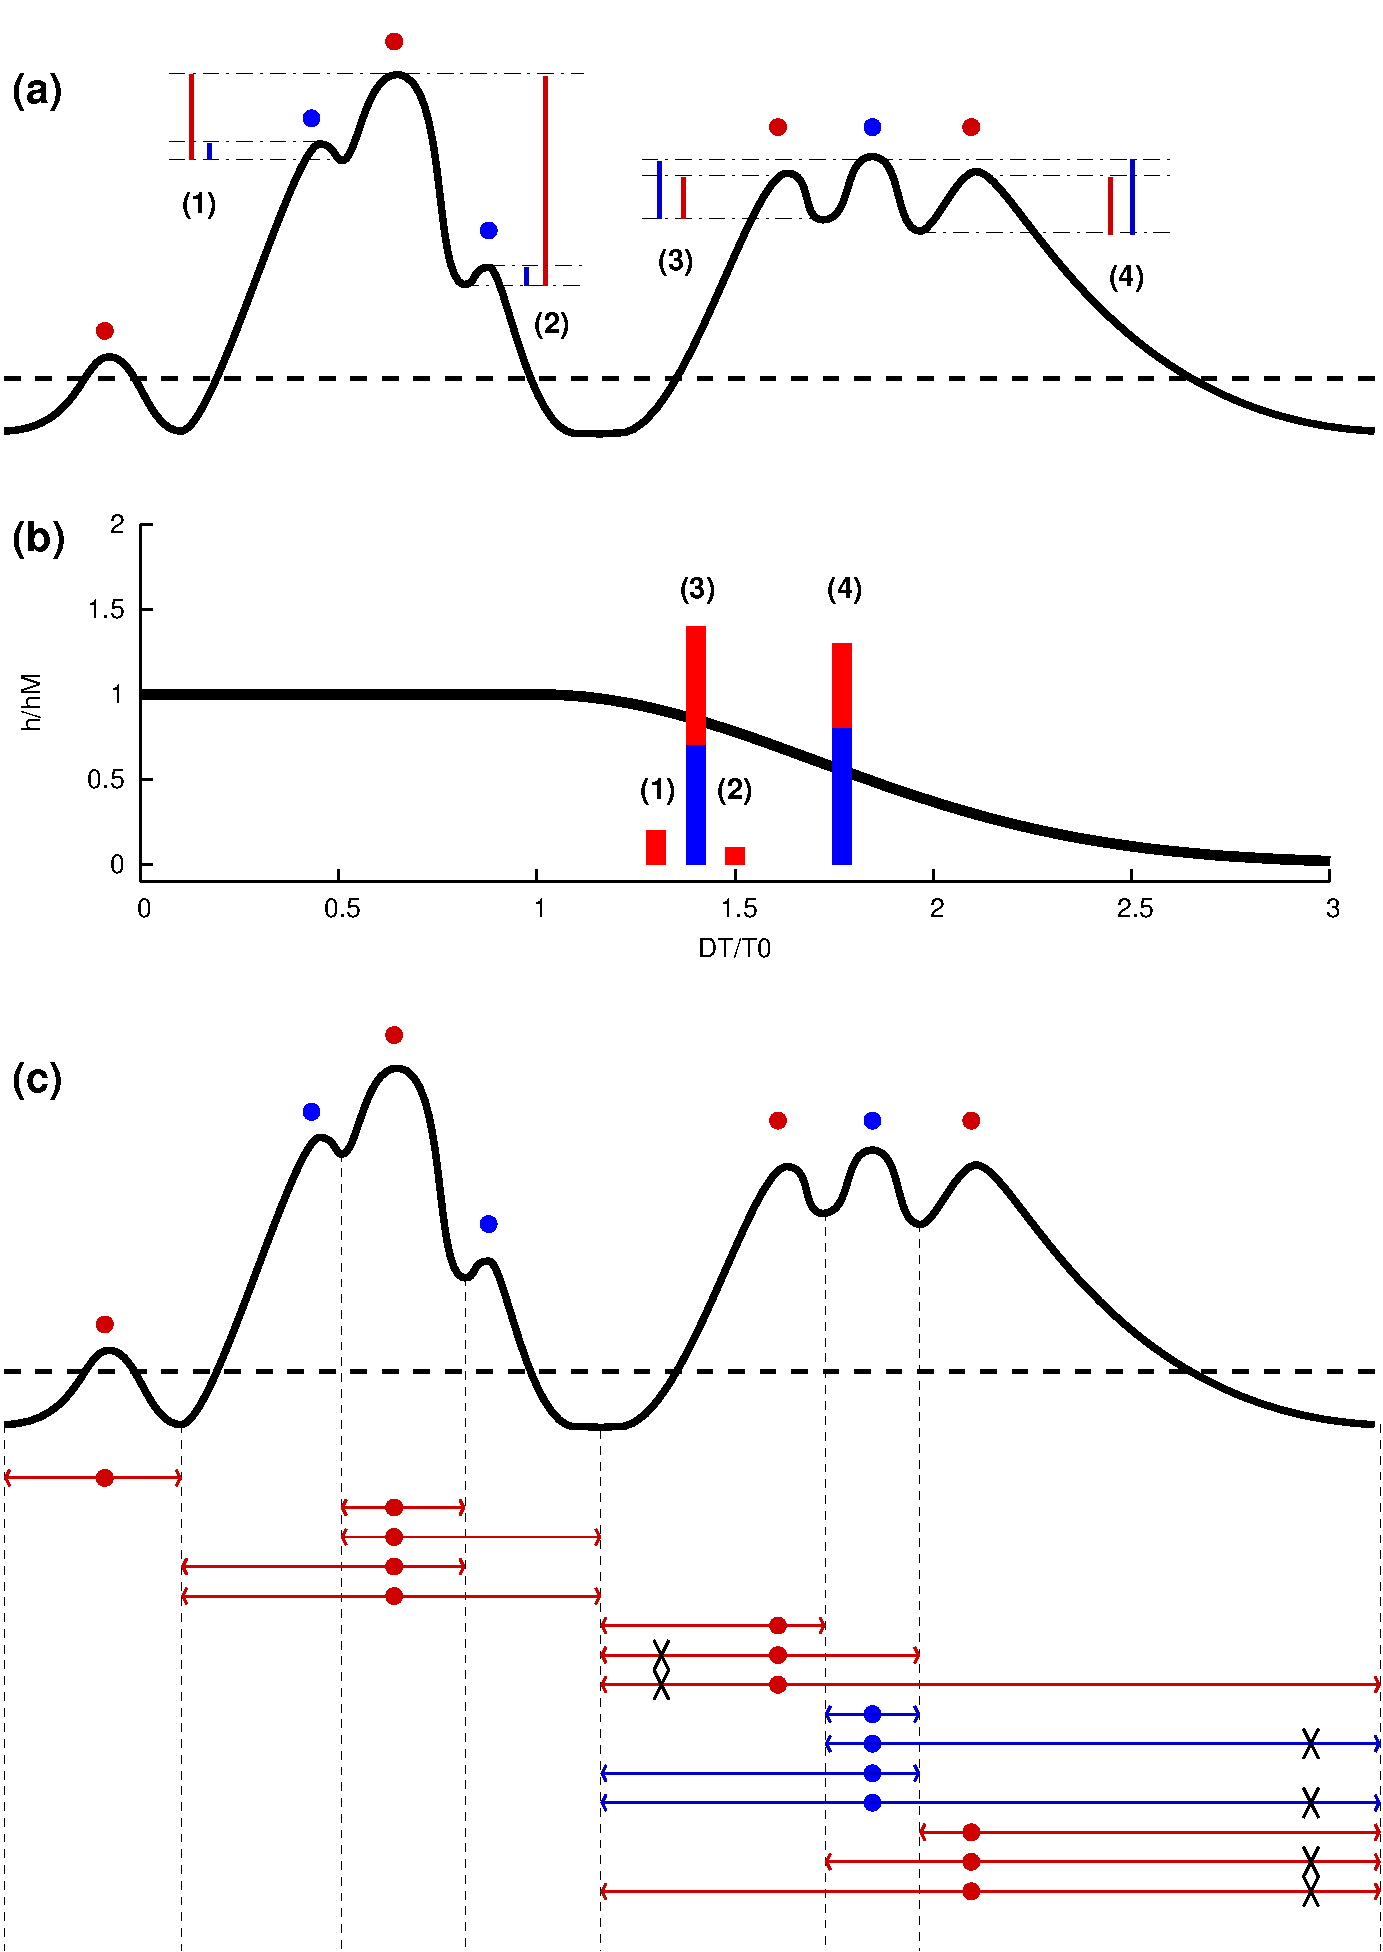
\includegraphics[width=5in]{window_rejection_separation.pdf}
\caption{\label{fg:separation}
Rejection of candidate windows based on the separation of distinct phases.
(a)~Heights of pairs of local maxima above their intervening minimum.
(b)~The black line represents the limiting value of $h/h_M$.  Vertical bars represent
$h/h_M$ for each pair of maxima.  Their position along the horizontal axis is
given by the time separation $\Delta T$ between the maxima of each pair.  The
color of the bar is given by the color of the seed maximum corresponding to $h_M$.  Bars whose height
exceeds the line represent windows to be rejected.
(c)~The windows that have been rejected by this criterion are indicated by black
crosses.
}
\end{figure}

\begin{figure}
\center 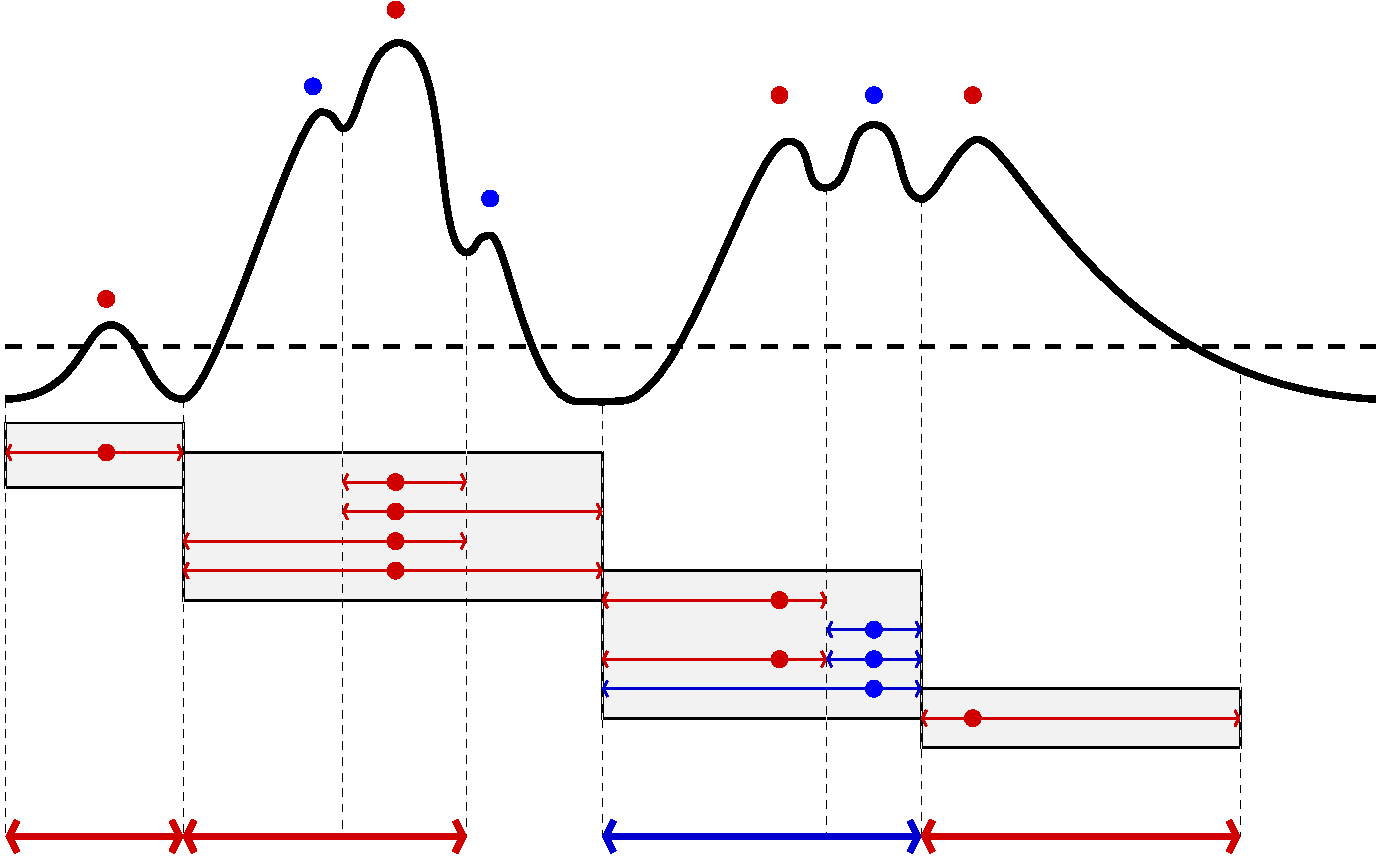
\includegraphics[width=5in]{window_overlap.pdf}
\caption{\label{fg:phaseD}
The selection of the best non-overlapping window
combinations.  Each grey box represents a distinct group of windows.
Non-overlapping subsets of windows are shown on separate lines.  Only one
line from within each group will be chosen, the one corresponding to the
highest weighted score.  The resulting optimal set
of data windows is shown by thick arrows.}
\end{figure}

\section{Time dependence of user parameters}
A subset of the FLEXWIN parameters from Table~\ref{tb:params} are time-dependent (where time is measured along the seismogram).  This feature enables the user to exercise fine control of the windowing algorithm.  The user can modulate the time-dependence of these parameters by editing the {\tt set\_up\_criteria\_arrays} subroutine in the {\tt user\_functions.f90} file.  This subroutine is called after the seismograms have been read in, and the following variables have been set: 
\begin{description}
\item[{\tt npts, dt, b}]  Number of points, time step, time of first point with respect to the reference time of both seismograms.  The observed and synthetic seismograms should have identical values of these three quantities.
\item[{\tt evla, evlo, evdp, stla, stlo}] Event latitude, event longitude, event depth (km), station latitude, station longitude, read from the observed seismogram.
\item[{\tt azimuth, backazimuth, dist\_deg, dist\_km}]  Calculated from the event and station locations above.
\item[{\tt kstnm, knetwk, kcmpnm}] Station name, network name, component name, read from the observed seismogram.
\item[{\tt num\_phases, ph\_names, ph\_times}] Number, names and arrival times of standard seismic phases calculated through IASPEI91 using the event depth and epicentral distance.
\end{description}

The {\tt set\_up\_criteria\_arrays} subroutine first sets up non time-modulated versions of the time-dependent parameters using a simple loop over time:
{\small
\begin{verbatim}
! -----------------------------------------------------------------
! This is the basic version of the subroutine - no variation with time
! -----------------------------------------------------------------
  do i = 1, npts
    time=b+(i-1)*dt
    DLNA_LIMIT(i)=DLNA_BASE
    CC_LIMIT(i)=CC_BASE
    TSHIFT_LIMIT(i)=TSHIFT_BASE
    STALTA_W_LEVEL(i)=STALTA_BASE
    S2N_LIMIT(i)=WINDOW_AMP_BASE
  enddo
\end{verbatim}
}
It is then up to the user to modulate these values for the specific problem at hand.  For example, should the user want to discourage the algorithm from picking windows beyond the end of the first surface wave-train $R1$, the following lines should be added to the {\tt user\_functions.f90} file to raise the water level on the STA:LTA waveform by a factor of ten:
{\small
\begin{verbatim}
 ! --------------------------------
 ! Set approximate end of rayleigh wave arrival
 R_vel=3.2
 R_time=dist_km/R_vel
 ! --------------------------------
 ! modulate criteria in time
 do i = 1, npts
   time=b+(i-1)*dt
   if (time.gt.R_time) then
     STALTA_W_LEVEL(i)=STALTA_BASE*10.0     
   endif
 enddo
\end{verbatim}
}
Should the user want the algorithm to be less stringent in its requirements for the cross-correlation fit for the surface wave portion of the seismograms, and allow a greater travel-time lag for deeper events, the required lines could be:
{\small
\begin{verbatim}
 ! --------------------------------
 ! Set approximate end of rayleigh wave arrival
 R_vel=3.2
 R_time=dist_km/R_vel
 ! --------------------------------
 ! Set approximate start of love wave arrival
 Q_vel=4.2
 Q_time=dist_km/Q_vel
 ! --------------------------------
 ! modulate criteria in time
 do i = 1, npts
   time=b+(i-1)*dt
   ! if we are in the surface wave times, then make the cross-correlation
   ! criterion less severe
   if (time.gt.Q_time .and. time.lt.R_time) then
     CC_LIMIT(i)=0.9*CC_LIMIT(i)
   endif
   ! --------------------------------
   ! modulate criteria according to event depth
   !
   ! if an intermediate depth event
   if (evdp.ge.70 .and. evdp.lt.300) then
     TSHIFT_LIMIT(i)=TSHIFT_BASE*1.4
   ! if a deep event
   elseif (evdp.ge.300) then
     TSHIFT_LIMIT(i)=TSHIFT_BASE*1.7
   endif
 enddo
 \end{verbatim}
}
 The above examples illustrate the power of the {\tt user\_functions.f90} file.  The user can choose to include/exclude any portion of the seismogram, and to make the rejection criteria for windows more or less stringent on any other portion of the seismogram.  All the seismogram-dependent variables whose values are known when the {\tt set\_up\_criteria\_arrays} subroutine is executed may be used to inform these choices, leading to an infinite number of windowing possibilities.  The careful user will use knowledge of the properties of the observed data set, the limitations of the synthetic waveforms, and the final use to which the selected windows will be put in order to tailor the subroutine to the needs of each study.  
 
 For a given set of data and synthetics, the {\tt PAR\_FILE} and {\tt user\_functions.f90} files uniquely determine the windowing results.

\subsection{Examples of user functions\label{ap:user_fn}}

%As concrete examples of how the time dependence of the tuning parameters can be exploited, we present here the functional forms of the time dependencies used for the three example tomographic scenarios (global, Japan and southern California) described in \cite{MaggiEtal2009}.
Here we present the time dependencies of tuning parameters used for three tomographic scenarios \citep{MaggiEtal2009}: global, Japan and southern California.
In each example we use predicted arrival times derived from 1D Earth models to help modulate certain parameters. Note, however, that the actual selection of individual windows is based on the details of the waveforms, and not on information from 1D Earth models.

\subsubsection{Global scenario\label{ap:user_global}}

In the following, $h$ indicates earthquake depth, $t_Q$ indicates the approximate start of the Love wave predicted by a group wave speed of 4.2~\kmps, and $t_R$ indicates the approximate end of the Rayleigh wave predicted by a group wave speed of 3.2~\kmps. In order to reduce the number of windows picked beyond R1, and to ensure that those selected beyond R1 are a very good match to the synthetic waveform, we raise the water level on the STA:LTA waveform and impose stricter criteria on the signal-to-noise ratio and the waveform similarity after the approximate end of the surface-wave arrivals.  We allow greater flexibility in cross-correlation time lag $\Delta\tau$ for intermediate depth and deep earthquakes.  We lower the cross-correlation value criterion for surface-waves in order to retain windows with a slight mismatch in dispersion characteristics.

We therefore use the following time modulations:
\begin{align}
w_E(t) & =
  \begin{cases}
    w_E \text{$t \leq t_R$} ,\\
    2 w_E \text{$t > t_R$},
  \end{cases}
\\
r_0(t) & = 
  \begin{cases}
    r_0 & \text{$t \leq t_R$}, \\
    10r_0 & \text{$t > t_R$} ,
  \end{cases}
\\
\mathrm{CC}_0(t) & = 
  \begin{cases}
    \mathrm{CC}_0 & \text{$t \leq t_R$}, \\
    0.9 \mathrm{CC}_0 & \text{$t_Q < t \leq t_R$}, \\
    0.95 & \text{$t > t_R$} ,
  \end{cases}
\\
\Delta\tau_0(t) & = 
  \begin{cases}
    \begin{cases}
      \tau_0 & \text{$t \leq t_R$}, \\
     \tau_0/3 & \text{$t > t_R$} ,
    \end{cases}
    & \text{$h \leq$ 70~km} \\
    1.4\tau_0 & \text{70~km $< h <$ 300~km}, \\
    1.7\tau_0 & \text{$h \geq$ 300~km},
  \end{cases}
  \\
\Delta \ln A_0(t) & = 
  \begin{cases}
    \Delta \ln A_0 & \text{$t \leq t_R$}, \\
    \Delta \ln A_0/3 & \text{$t > t_R$} .
  \end{cases}
\end{align}

%--------------------------

\subsubsection{Japan scenario\label{ap:user_japan}}
In the following, $t_P$ and $t_S$ denote the start of the time windows for $P$- and $S$ waves, as predicted by the 1-D IASPEI91 model \citep{KennettEngdahl1991}, and $t_{R1}$ indicates the end of the surface-wave time window.  For the \trange{24}{120} data, we consider the waveform between the start of the $P$ wave to the end of the surface-wave.  We therefore modulate $w_E(t)$ as follows:

%
\begin{align}
w_E(t) & =
  \begin{cases}
    10 w_E & \text{$t < t_P$}, \\
    w_E & \text{$t_P \le t \leq t_{R1}$}, \\
    10 w_E & \text{$t > t_{R1}$}.
  \end{cases}
\end{align}

For the \trange{6}{30} data, the fit between the synthetic and observed surface-waves is expected to be poor, as the 3D model used to calculate the synthetics cannot produce the required complexity. We therefore want to concentrate on body-wave arrivals only, and avoid surface-wave windows altogether by modulating $w_E(t)$ as follows:
%
\begin{align}
w_E(t) & =
  \begin{cases}
    10 w_E & \text{$t < t_P$}, \\
    w_E & \text{$t_P \le t \leq t_S$}, \\
    10 w_E & \text{$t > t_S$}.
  \end{cases}
\end{align}

We use constant values of $r_0(t)=r_0$, $\mathrm{CC}_0(t)=\mathrm{CC}_0$ and $\Delta \ln A_0(t)=\Delta \ln A_0$ for both period ranges.  In order to allow greater flexibility in cross-correlation time lag $\Delta\tau$ for intermediate depth and deep earthquakes we use:

\begin{align}
\Delta\tau_0(t) & = 
  \begin{cases}
    0.08 \text{$t_P$} & \text{$h \leq$ 70~km}, \\
    \max(0.05 \text{$t_P$}, 1.4\tau_0) & \text{70~km $< h <$ 300~km}, \\
    \max(0.05 \text{$t_P$}, 1.7\tau_0) & \text{$h \geq$ 300~km}.
  \end{cases}
\end{align}
%--------------------------

\subsubsection{Southern California scenario\label{ap:user_socal}}

In the following, $t_P$ and $t_S$ denote the start of the time windows for the crustal P wave and the crustal S wave, computed from a 1D layered model appropriate to Southern California \citep{Wald95}.  The start and end times for the surface-wave time window, $t_{R0}$ and $t_{R1}$, as well as the criteria for the time shifts $\Delta\tau_0(t)$, are derived from formulas in \cite{KomatitschEtal2004}. The source-receiver distance (in km) is denoted by $\Delta$.

%CHT modified

For the \trange{6}{30} and \trange{3}{30} data, we use constant values of $r_0(t)=r_0$, $\mathrm{CC}_0(t)=\mathrm{CC}_0$, $\Delta\tau_0(t)=\Delta\tau_0$, and $\Delta \ln A_0(t)=\Delta \ln A_0$. We exclude any arrivals before the $P$ wave and after the Rayleigh wave. This is achieved by the box-car function for $w_E(t)$:  
%
\begin{align}
w_E(t) & =
  \begin{cases}
    10 w_E & \text{$t < t_P$}, \\
    w_E & \text{$t_P \le t \leq t_{R1}$}, \\
    10 w_E & \text{$t > t_{R1}$},
  \end{cases}
\end{align}
%For the \trange{6}{30} data, we exclude any arrivals before the $P$ wave and reduce the number of windows picked beyond R1 by modulating $w_E(t)$.  We use constant values of $r_0(t)=r_0$, $\mathrm{CC}_0(t)=\mathrm{CC}_0$ and $\Delta \ln A_0(t)=\Delta \ln A_0$, but modulate the cross-correlation time lag criterion so that it is less strict at larger epicentral distances and for surface-waves.  We therefore use:  
%
%\begin{align}
%w_E(t) & =
%  \begin{cases}
%    10 w_E & \text{$t < t_P$}, \\
%    w_E & \text{$t_P \le t \leq t_{R1}$}, \\
%    2 w_E & \text{$t > t_{R1}$},
%  \end{cases}
%\\
%\Delta\tau_0(t) & = 
%  \begin{cases}
%    3.0 + \Delta/80.0 & \text{$t \le t_{R0}$}, \\
%    3.0 + \Delta/50.0 & \text{$t > t_{R0}$},
%  \end{cases}
%\end{align}

For the \trange{2}{30} data, we avoid selecting surface-wave arrivals as the 3D model used to calculate the synthetics cannot produce the required complexity. The water-level criteria then becomes:

\begin{align}
w_E(t) & =
  \begin{cases}
    10 w_E & \text{$t < t_P$}, \\
    w_E & \text{$t_P \le t \leq t_S$}, \\
    10 w_E & \text{$t > t_S$}.
  \end{cases}
%\\
%\Delta\tau_0(t) & = \Delta\tau_0.
\end{align}

%-----------------------

\subsection{Time intervals for signal-to-noise calculations}

If the parameter {\tt DATA$\_$QUALITY = .true.} in the {\tt PAR$\_$FILE}, then the {\tt user\_functions.f90} file requires the specification of four times that define the ``noise'' and ``signal'' time intervals.  For example, the default {\tt user\_functions.f90} file contains these lines:
%
\begin{verbatim}
  ! these values will be used for signal2noise calculations
  if (DATA_QUALITY) then
    noise_start=b
    noise_end=ph_times(1)-WIN_MAX_PERIOD
    signal_start=noise_end
    signal_end=b+(npts-1)*dt
  endif
\end{verbatim}
%
The use of all four variables allows provides the flexibility of choosing these time intervals.  (For example, the start of the noise does not need to be the beginning of the seismogram. Or the start of the signal does not have to coincide with the end of the noise.)

%-----------------------


\section{Tuning considerations}
FLEXWIN is not a black-box application and should not be applied blindly
to any given dataset or tomographic scenario.  The data windowing required by
any given problem will differ depending on the inversion method, the scale of
the problem (local, regional, global), the quality of the data set, the quality of the model,
and the accuracy of the method used to calculate the synthetic seismograms.  The user
must configure and tune the algorithm for the given problem.  Here we
discuss general considerations the user should bear in mind.

We suggest the following as a practical starting sequence for tuning the algorithm.
Keep in mind that this process may need to be repeated and refined several times before
converging on the optimal set of parameters for a given problem and data-set.

$T_{0,1}$ : In setting the corner periods of the bandpass filter, the
user is deciding on the frequency content of the information to be used in the
tomographic problem.  Values of these corner periods should reflect the
information content of the data, the quality of the Earth model and the
accuracy of the simulation used to generate the synthetic seismogram.  The
frequency content in the data depends on the spectral characteristics of the
source, on the instrument responses, and on the attenuation
characteristics of the medium. As $T_{0,1}$ depend on the source and station
characteristics, which may be heterogeneous in any given data-set, these filter
periods can be modified dynamically by constructing an appropriate user
function (e.g. {\em if station is in list of stations with instrument X then
reset T0 and T1 to new values}).

$r_{P,A}$ : In setting the signal-to-noise ratios for the entire seismogram, the
user is applying a simple quality control on the data.  Note that these criteria 
are applied after filtering.  No windows will be defined on data that fail this
quality control.  

$w_E(t)$ : For a constant signal the short-term average long-term average ratio, $E(t)$,
converges to a constant value when
the length of the time-series is greater than the effective averaging length of
the long-term average.  This value is 0.08 for the short-term average long-term average ratio used in FLEXWIN (it has a small dependence on $T_0$, which can be ignored in most applications).  We suggest the user start with a constant
level for $w_E(t)$ equal to this convergence value.  The time dependence of
$w_E(t)$ should then be adjusted to exclude those portions of the waveform the
user is not interested in, by raising $w_E(t)$ (e.g. to exclude the fundamental
mode surface-wave: {\em if t $>$ fundamental mode surface-wave arrival time then set $w_E(t)=1$}).  
We suggest finer adjustments to $w_E(t)$ be made after $r0(t)$,
$CC_0(t)$, $\Delta T_0(t)$ and $\Delta \ln A_0(t)$ have been configured.

$r_0(t)$, $\mathrm{CC}_0(t)$, $\Delta \tau_{\rm ref}$, $\Delta
\tau_0(t)$, $\Delta \ln A_{\rm ref}$ and $\Delta \ln A_0(t)$ : These parameters ---
window signal-to-noise ratio, normalized cross-correlation value between
observed and synthetic seismograms, cross-correlation time lag, and amplitude
ratio --- control the degree of well-behavedness of the data within accepted
windows.  The user first sets constant values for these four parameters, then
adds a time dependence if required.  Considerations that should be taken into
account include the quality of the Earth model used to calculate the synthetic
seismograms, the frequency range, the dispersed nature of certain arrivals (e.g.
{\em for t corresponding to the group velocities of surface-waves, reduce
$CC_0(t)$}), and {\em a priori} preferences for picking certain small-amplitude seismic phases
(e.g. {\em for t close to the expected arrival for $P_{\rm diff}$, reduce $r_0(t)$}).  
$\Delta \tau_{\rm ref}$ and $\Delta \ln A_{\rm ref}$ should be set to zero at first, and only
reset if the synthetics contain a systematic bias in traveltimes or amplitudes.


$c_{0-4}$ : These parameters control the process by which the suite of all possible data windows is pared down using criteria on the shape of the STA:LTA $E(t)$ waveform alone.  We suggest the user start by setting these values to those used in our global example (see Table~\ref{tb:example_params}).  Subsequent minimal tuning should be performed by running the algorithm on a subset of the data and closely examining the lists of windows rejected at each stage to make sure the user agrees with the choices made by the algorithm.  

$w_{\mathrm{CC}}$, $w_{\rm len}$ and $w_{\rm nwin}$ : These parameters control the overlap resolution stage of the algorithm.  Values of $w_{\mathrm{CC}}= w_{\rm len} = w_{\rm nwin} = 1$ should be reasonable for most applications.

The objective of the tuning process summarized here should be to maximize the selection of windows around desirable features in the seismogram, while minimizing the selection of undesirable features.
Of course, the desirability or undesirability of a given feature is subjective, and it depends on how the user subsequently intends to use the information contained within the data windows.

